\documentclass{article}
\usepackage[utf8]{inputenc}
\usepackage{tikz}
\usetikzlibrary{snakes}

\begin{document}
\thispagestyle{empty}
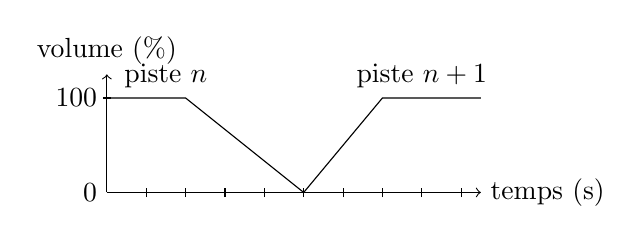
\begin{tikzpicture}[xscale=0.5,yscale=0.6]
\draw[->] (0,0) -- (0,2.5);
\draw (-0.1,2) -- (0.1,2);
\draw (0,2) node[anchor=east]{100};
\draw (0,0) node[anchor=east]{0};
\draw[->] (0,0) -- (9.5,0);
\foreach \x in {1,2,3,4,5,6,7,8,9} \draw (\x,-0.1) -- (\x,0.1);
\draw (0,2.5) node[anchor=south]{volume (\%)};
\draw (9.5,0) node[anchor=west]{temps (s)};
\draw (0,2) -- (2,2) -- (5,0);
\draw (5,0) -- (7,2) -- (9.5,2);
\draw (1.5,2) node[anchor=south]{piste $n$};
\draw (8,2) node[anchor=south]{piste $n+1$};
\end{tikzpicture}
\end{document}
